\documentclass[10pt,twocolumn,letterpaper]{article}

\usepackage[pdf]{pstricks}
\usepackage{cvpr}
\usepackage{times}
\usepackage{epsfig}
\usepackage{graphicx}
\usepackage{amsmath}
\usepackage{amssymb,amsfonts}
\usepackage{bm}
\usepackage{xcolor}

% Include other packages here, before hyperref.

\usepackage{algorithm}
\usepackage{algorithmic}

%--------------------------------- Variable representation --------------------------------------------%
\DeclareMathOperator*{\E}{\mathbb{E}}
\providecommand{\trace}[1]{\ensuremath{tr}\{#1\}}% expectation operator
\providecommand{\cov}[2]{{\ensuremath{cov}}\{#1,#2\}}% covariance operator, \cov{x} {y}
\providecommand{\var}[1]{{\ensuremath{var}}\{#1\}}% variance operator
\providecommand{\re}[1]{{\ensuremath{Re}}\{#1\}}% real part
\providecommand{\ve}[1]{{\bm{#1}}} %
\providecommand{\mat}[1]{{\bm{#1}}} %
\providecommand{\est}[1]{{\widetilde {#1}}}
\DeclareMathOperator{\Real}{\mathbb{R}}
\DeclareMathOperator{\Complex}{\mathbb{C}}

\newcommand{\stateb}{\STATE \textbullet~}

% If you comment hyperref and then uncomment it, you should delete
% egpaper.aux before re-running latex.  (Or just hit 'q' on the first latex
% run, let it finish, and you should be clear).
\usepackage[pagebackref=true,breaklinks=true,letterpaper=true,colorlinks,bookmarks=false]{hyperref}

% \cvprfinalcopy % *** Uncomment this line for the final submission

\def\cvprPaperID{***} % *** Enter the CVPR Paper ID here
\def\httilde{\mbox{\tt\raisebox{-.5ex}{\symbol{126}}}}

% Pages are numbered in submission mode, and unnumbered in camera-ready
\ifcvprfinal\pagestyle{empty}\fi
\begin{document}

%%%%%%%%% TITLE
\title{Weakly supervised super resolution for plant and root imaging}

\author{Jose Francisco Ruiz-Munoz, Alina Zare \\
University of Florida, Department of Electrical and Computer Engineering, Gainesville, FL, USA\\
{\tt\small jruizmunoz@ufl.edu, azare@ece.ufl.edu}
% For a paper whose authors are all at the same institution,
% omit the following lines up until the closing ``}''.
% Additional authors and addresses can be added with ``\and'',
% just like the second author.
% To save space, use either the email address or home page, not both
% \and
% Second Author\\
% Institution2\\
% First line of institution2 address\\
%{\tt\small secondauthor@i2.org}
}

\maketitle
%\thispagestyle{empty}

%%%%%%%%% ABSTRACT
\begin{abstract}
   Plant phenotyping applications frequently require handling poor quality data due to non-controlled environmental conditions or difficulty in designing high-resolution sensors for some tasks. In this study, we propose a super-resolution (SR) algorithm that transforms low-resolution (LR) images into higher-quality images based on a generative adversarial network (GAN). Our scheme includes a network that generates images with two purposes: i) fooling a discriminator trained to detect real high-resolution (HR) images, and ii) increasing the classification performance. Our results show that the proposed approach allows creating super-resolved images appropriated for leaf-disease-based classification and imaging X-ray back-scatter scans of roots.
\end{abstract}

%%%%%%%%% BODY TEXT
\section{Introduction}

\texttt{[THIS SECTION IS IN PROGRESS... MAIN IDEAS ARE LISTED BELOW]}\\

\texttt{[MOTIVATION]}\\
High-throughput image-based phenotyping facilitates the measurement of features of the plants required for crop production analysis and the design of ecological models. This technology consists of tools of hardware and software that allows the acquisition and processing of the target biophysical data. Tasks that traditionally are carried out by visual inspection can be made efficiently by using standard and hyper-spectral cameras~\cite{Fahlgren2015}. However, these sensors usually have resolution limitation or are not appropriate to acquire a certain type of data, e.g., below-ground data. In this paper, we address the resolution problem by developing a weakly supervised super-resolution (SR) algorithm and apply it to two tasks:  i) disease classification and ii) root imaging based on a novel X-ray backscatter technology.

\texttt{[DIGITAL SIGNAL PROCESSING AND MACHINE LEARNING FOR ROOTS PHENOTYPING]}

Digital signal processing (DSP) and machine learning (ML) techniques have been applied in phenotyping tasks for segmentation and classification of images. In \cite{Ramcharan2017}, a method for disease detection based on a deep learning model is proposed.

Deep-learning has become very popular in the machine learning community but has not been extensively studied for plant phenotyping applications~\cite{Ubbens2017}.

Handling low-quality images and image acquisition under non-controlled conditions is a challenge for automatic plant phenotyping.

Phenotyping roots in situ is a challenging task since most of the cases it is difficult to distinguish them from their surroundings~\cite{Tabb2018}. More advanced non-invasive techniques include electrical capacitance and ground-penetrating radar. However, these sensors still have restrictions in depth and resolution~\cite{Araus2014}.

\texttt{[SUPER RESOLUTION]}

The SR task consists of recovering HR images from low-resolution (LR) images. Many SR approaches can be found in the DSP and ML literature. Applications such as medical diagnostic heavily rely on high-quality images~\cite{Zhang2012}. This is an inherently ill-posed problem, i.e., no unique solution exists~\cite{Hui2018}. Therefore, the SR methods require regularization terms to constrain the search space.

Super-resolution algorithms promote the development of new alternatives to sense data, such as X-ray based sensors, since efficient algorithms can help to overcome weakness in hardware.

A previous study about SR of plant images is described in \cite{Yamamoto2017}.

The loss function of an SR problem is usually the mean squared error (MSE) between the estimated SR image and the original HR image plus a regularization term~\cite{Ledig2017}. MSE minimization might not avoid visual artifacts. Some SR methods require pairs of LR-HR examples~\cite{Zeyde2012}, which is a practical disadvantage. 

A general adversarial network (GAN) can be used to learn a transformation between two domains~\cite{Hong2018}. In \cite{Giuffrida2017}, GANs are used for data augmentation in plant phenotyping.

\texttt{[BRIEF DESCRIPTION OF THE PROPOSED METHOD]}

% ``Here high-throughput image-based phenotyping is defined as technology that can minimally image hundreds of plants per day.'' ``The goal of plant imaging and analysis is to measure the physiological, growth, development, and other phenotypic properties of plants through automated processes.'' ``Digital camera technology has become relatively inexpensive and ubiquitous, leading to a recent surge in high-throughput phenotyping systems that utilize plant imaging to capture data''~\cite{Fahlgren2015}.


%``Single image super-resolution (SISR) is a classical problem in low-level computer vision, which reconstructs a high-resolution (HR) image from a low-resolution (LR) image. Actually, an infinite number of HR images can get the same LR image by downsampling. Hence, the SR problem is inherently ill-posed and no unique solution exists''~\cite{Hui2018}.

% ``The optimization target of supervised SR algorithms is commonly the minimization of the mean squared error (MSE) between the recovered HR image and the ground truth''~\cite{Ledig2017}.

% ``How can we achieve unsupervised domain adaptation without relying on the assumption that the source and target domains share a same prediction function in a domain-invariant feature space? In this work, we propose a principled approach to model the residual in the feature space between the source and target domain. We train a deep residual net to transform the feature maps of source domain images to appear as if they were sampled from the target domain while maintaining their semantic spatial layouts. We propose a novel Generative Adversarial Network (GAN)-based architecture that is capable of learning such a transformation in an unsupervised manner. Note, we do not require corresponding image pairs from the two domains, which are not available in practice''~\cite{Hong2018}.

% ``Image recognition offers both a cost effective and scalable technology for disease detection. New deep learning models offer an avenue for this technology to be easily deployed on mobile devices''~\cite{Ramcharan2017}.

% ``Segmentation is a challenging problem in this context because the root and non-root regions share similar features''~\cite{Tabb2018}.

% ``Many applications require resolution enhancement of images acquired by low-resolution sensors (e.g. for high-resolution displays), while minimizing visual artifacts.'' ``Pairs of matching patches that form the training database''~\cite{Zeyde2012}.

% ``(SR) is a very active research topic in the image processing community. In practice, many tasks, such as astronomical observation and medical diagnostic rely on high quality images for reliable and accurate analysis as well as prediction. However, in many practical situations, due to the inherent limitations of the optical system or other factors, the observed images are often of low resolution, thus limiting the subsequent tasks based on them.'' ``The minimum mean square error (MMSE) criteria are used for estimating the HR image. A Markov chain Monte Carlo- based sampling algorithm is presented for obtaining the MMSE solution. The proposed method cannot only enjoy the benefits offered by the flexible prior, but also has the advantage of making use of the probabilistic modeling to perform a posterior mean estimation, thus is less sensitive to the local minima problem as the MAP solution. Experimental results indicate that the proposed method can generate competitive or better results than state-of-the-art SR algorithms''~\cite{Zhang2012}.

%-------------------------------------------------------------------------

\section{Methods}
% To draw NN http://alexlenail.me/NN-SVG/index.html

\subsection{Adversarial Networks}
%``The general idea behind this formulation is that it allows one to train a generative model $G$ with the goal of fooling a differentiable discriminator $D$ that is trained to distinguish super-resolved images from real images. With this approach our generator can learn to create solutions that are highly similar to real images and thus difficult to classify by $D$''.

A basic generative adversarial network (GAN) consists of two nets ---a generator $G,$ and a discriminator $D$. On the adversarial configuration, these two nets play opposite roles, i.e., on the one hand, $G$ aims at generating ``realistic-like fake data'' capable of fooling $D$, whereas $D$ is continuously trained to classify fake data from real data~\cite{Goodfellow2014}. This formulation is expressed as follows
\begin{eqnarray}
\label{eq:gan}
\begin{aligned}
& \min_G \max_D \E_{\ve{x} \sim p(\ve{x})}[\log D(\ve{x})]\\
& +\E_{\ve{z} \sim p(\ve{z})}[\log (1 - D(G(\ve{z})))]  
\end{aligned}
\end{eqnarray}
where $\ve{x}$ denotes a real sample, and $\ve{z}$ is the input of the generator, that depending on the problem might be random noise, a lower-resolution sample, or a version of a sample in other domain.

\subsection{Classification loss function}
The parameters of a two-class classifier $C$ at the image level can be found solving
\begin{eqnarray}
\label{eq:cnet}
\min_C \E_{\ve{x} \sim p(\ve{x|L_0})}[\log C(\ve{x})] +  \E_{\ve{x} \sim p(\ve{x|L_1})}[1-\log C(\ve{x})]
\end{eqnarray}
where $C$ outputs the probability that its input $x$ comes from the target class distribution $p(x|L_1)$ and not from the non-target class distribution $p(x|L_0),$ i.e., if $C(x)=1$ the classifier ensures that $x$ is a sample of the target class $L_1,$ on the other hand, $C(x)=0$ indicates that $x$ is a sample of the non-target class $L_0$.

\subsection{Weakly supervised adversarial network}

Our proposed method is illustrated in Fig.~\ref{fig:cgan}. The network is divided into three stages, i) $G$ that generates SR images from LR inputs, ii) $D$ that classifies HR images from SR images, and iii) $C$ that is our additional regularization to the traditional GAN, which allows enhancing relevant aspects in the generated images for classification purposes. 

\begin{figure}[h]
\begin{center}
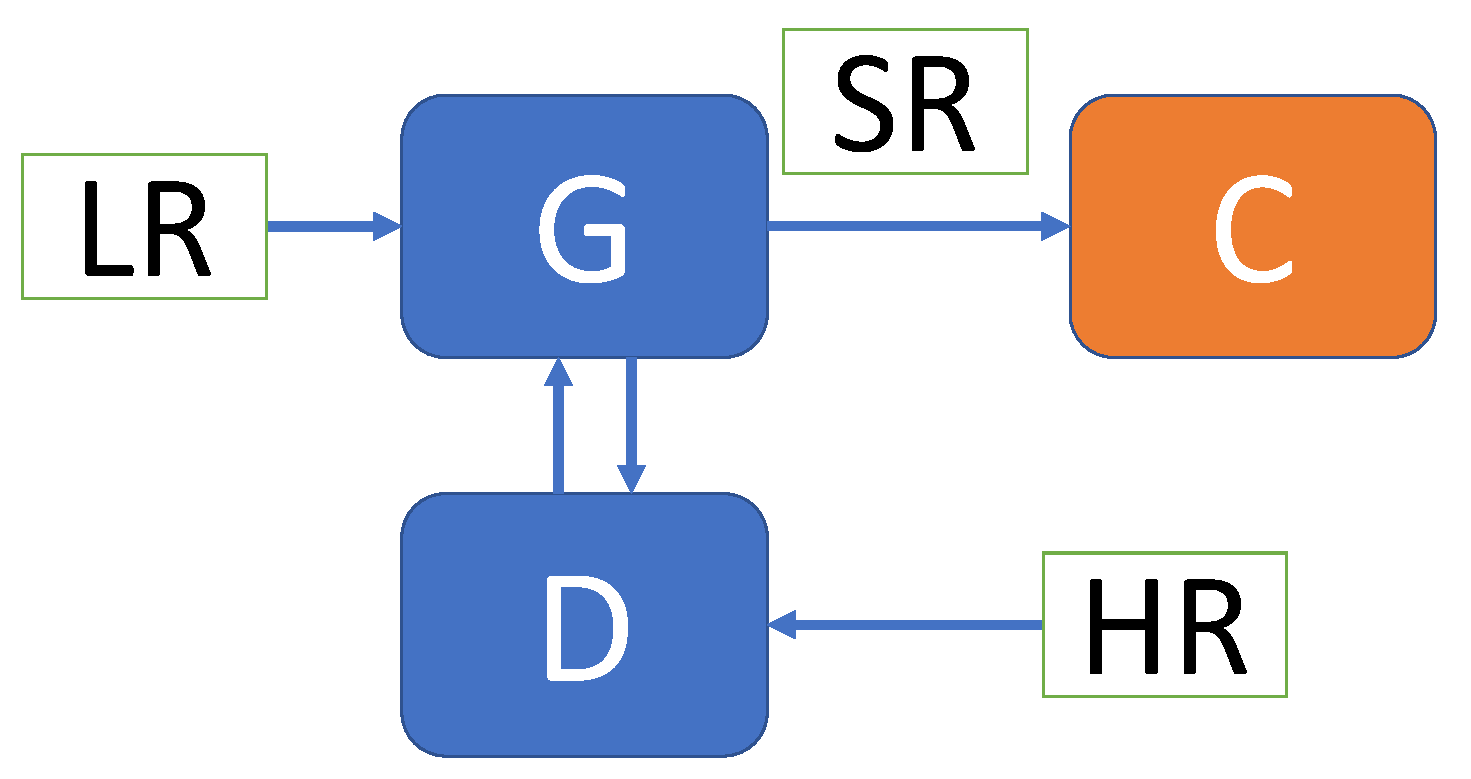
\includegraphics[scale=0.25]{cgan.pdf}
\end{center}
   \caption{Generation of SR images by an adversarial network. This method consists of three blocks: generator ($G$), discriminator ($D$), and classifier ($C$).}
\label{fig:cgan}
\end{figure}

Our proposed formulation is expressed as follows
\begin{eqnarray}
\label{eq:srcgan}
\footnotesize
\begin{aligned}
& \min_{C,G} \max_D \E_{\ve{z} \sim p(\ve{z|L_0})}[\log C(G(\ve{z}))] \\ & +  \E_{\ve{z} \sim p(\ve{z|L_1})}[1-\log C(G(\ve{z}))] \\ & + \E_{\ve{x} \sim p(\ve{x})}[\log D(\ve{x})] + \E_{\ve{z} \sim p(\ve{z})}[\log (1 - D(G(\ve{z})))].
\end{aligned}
\end{eqnarray}
Note that $G$ maps the labeled-LR data $z$ to a higher-resolution domain. Since we assume that the HR labels are unknown, the classifier is trained with the SR data. Algorithm~\ref{alg:srcgan} contains the pseudo-code of our method.

\begin{algorithm}[h]
    \caption{Minibatch gradient descent training of the \textbf{weakly supervised adversarial network}.}
    \label{alg:srcgan}
    \begin{algorithmic}
    \FOR{number of training iterations}
    \stateb Sample minibatch of $m$ samples $\{x_1,\ldots, x_m\}$ from HR data distribution $p(x)$.
    \stateb Sample minibatch of $m$ samples $\{y_1,\ldots, y_m\}$ from LR data distribution $p(y|L_0)$.
    \stateb Sample minibatch of $m$ samples $\{z_1,\ldots, z_m\}$ from LR data distribution $p(z|L_1)$.
    \stateb Update the classifier by descending its stochastic gradient
    \[\nabla_{\theta_c} \frac{1}{m} \sum_{i=1}^m \left[\log C(G(y_i)) + \log(1 - C(G(z_i))) \right]. \]
    \stateb Update the discriminator by descending its stochastic gradient
    \[
    \begin{aligned}
    \nabla_{\theta_d} \frac{1}{m} \sum_{i=1}^m \left[\log D(z_i) + \log(1- D(G(x_i))) \right. \\ \left. + \log(1- D(G(y_i))) \right].
    \end{aligned}
    \]
    \stateb Update the generator by descending its stochastic gradient
    \[
    \nabla_{\theta_{g}} \frac{1}{m} \sum_{i=1}^m \log(1- D(G(x_i)))+\log(1- D(G(y_i))).\]
    %\stateb Compute $m$ code-words $\{z_1,\ldots, z_m\}$ by $z_i = G(x_i)$
    \stateb Update the decoder by descending its stochastic gradient
    \ENDFOR
    \STATE The gradient-based updates can use any standard gradient-based learning rule.
    \end{algorithmic}
\end{algorithm}


Figure~\ref{fig:D_net} shows the architecture for $C$ and $D.$ We use the same architecture for both of them. Figure~\ref{fig:G_net} shows the generator architecture.

\begin{figure*}[h]
\begin{center}
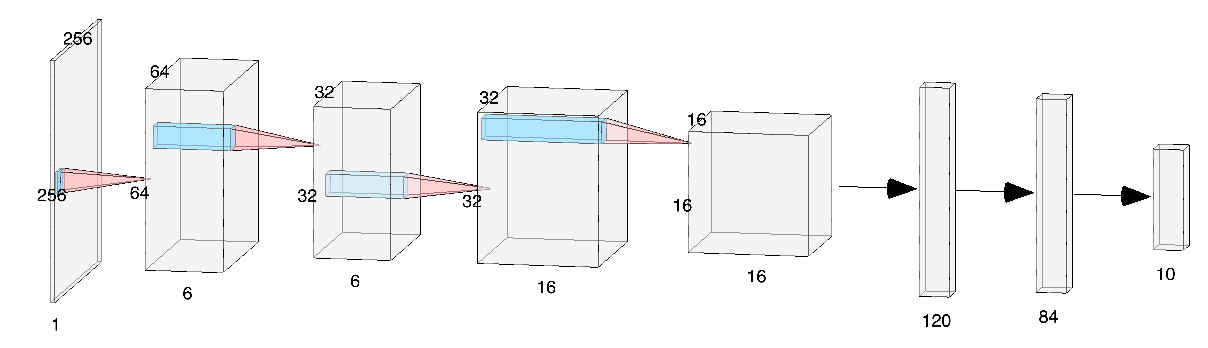
\includegraphics[scale=0.35]{D_net.png}
\end{center}
   \caption{Discriminator ($D$) and classifier ($C$) network. Same architecture is used for each one of them.}
\label{fig:D_net}
\end{figure*}

\begin{figure*}[h]
\begin{center}
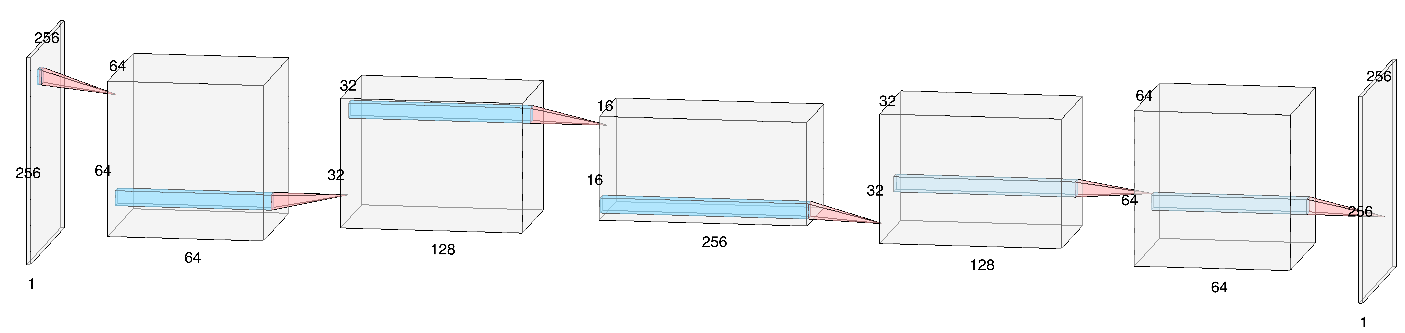
\includegraphics[scale=0.30]{G_net.png}
\end{center}
\label{fig:G_net}
\caption{Generator (G) network.}
\end{figure*}

%------------------------------------------------------------------------

\section{Experiments}

% \texttt{[THIS SECTION IS IN PROGRESS.  TABLES CONTAIN CLASSIFICATION ACCURACY ON HR, SR, AND LR DATA OF TWO DATASETS: LEAF-BASED DISEASE CLASSIFICATION AND CT SCANS CORES OF TURFACE AND ROOTS. FIGURES CONTAIN EXAMPLES OF IMAGES ON THESE DATASETS AND THE RESULTS OF THE METHOD APPLIED TO THE X-RAY BACKSCATTER SCANS.]}\\

We perform experiments on three datasets. The first one contains 3719 images (from PlantVillage project~\cite{Hughes2015}) of tomato leaves divided into two classes: Healthy (1592) and Bacteria (2127). The second dataset is formed by the images of the scans of two CT cores.  The third dataset consists of 8 buried-roots scans and 4 soil scans, which were acquired by the authors using a novel x-ray backscatter system. Note that our method requires labels of the LR images at image level. As gradient-based learning rule, we use the Adaptive Moment Estimation (Adam). 

\subsection{Disease Classification}
%\url{https://github.com/spMohanty/PlantVillage-Dataset}
We apply our method to an image-based plant disease classification task~\cite{Mohanty2016}. We consider the original grayscale images ($256\times 256$) of the PlantVillage dataset as HR data. We create the LR versions of this images by downsampling 2 (LR2x: $128\times 128$), 4 (LR4x: $64\times 64$), 8 (LR8x: $32\times 32$), and 16 (LR16x: $16\times 16$) times and upsampling them again to $256\times 256$ by a bicubic interpolation. Table~\ref{tab:results} shows the classification accuracy in a test set (200 images per class) obtained when trained the classifier only with HR data (baseline) and when trained with LR data and with SR data (SR2x, SR4x, SR8x, and SR16x applied to LR2x, LR4x, LR8x, and LR16x, respectively). Figure~\ref{fig:srimages} contains some examples of HR, LR and SR of each class (Tomato - healthy and Tomato - bacterial spot).

\begin{table}[h]
\caption{Classification performance on the PlantVillage dataset applied to a test set.}
\label{tab:results}
\centering
\begin{tabular}{|l|c|c|c|}
\hline
  Scale   & Accuracy & TP & TN \\
\hline
\hline
HR & 97.5 & 95.0 & 100 \\
\hline
LR2x & 90.5 & 81.0 & 100 \\
SR2x & \textbf{97.0} & \textbf{94.0} & 100 \\
\hline
LR4x & 68.3 & 36.5 & 100 \\
SR4x & \textbf{94.7} & \textbf{89.5} & 100 \\
\hline
LR8x & 51.0 & 02.0 & \textbf{100} \\
SR8x & \textbf{81.3} & \textbf{87.5} & 75.0 \\
\hline
LR16x & 50.0 & 00.0 & \textbf{100} \\
SR16x & \textbf{59.7} & \textbf{94.5} & 25.0 \\
\hline
\end{tabular}
\end{table}

\begin{figure*}[h]
\begin{center}
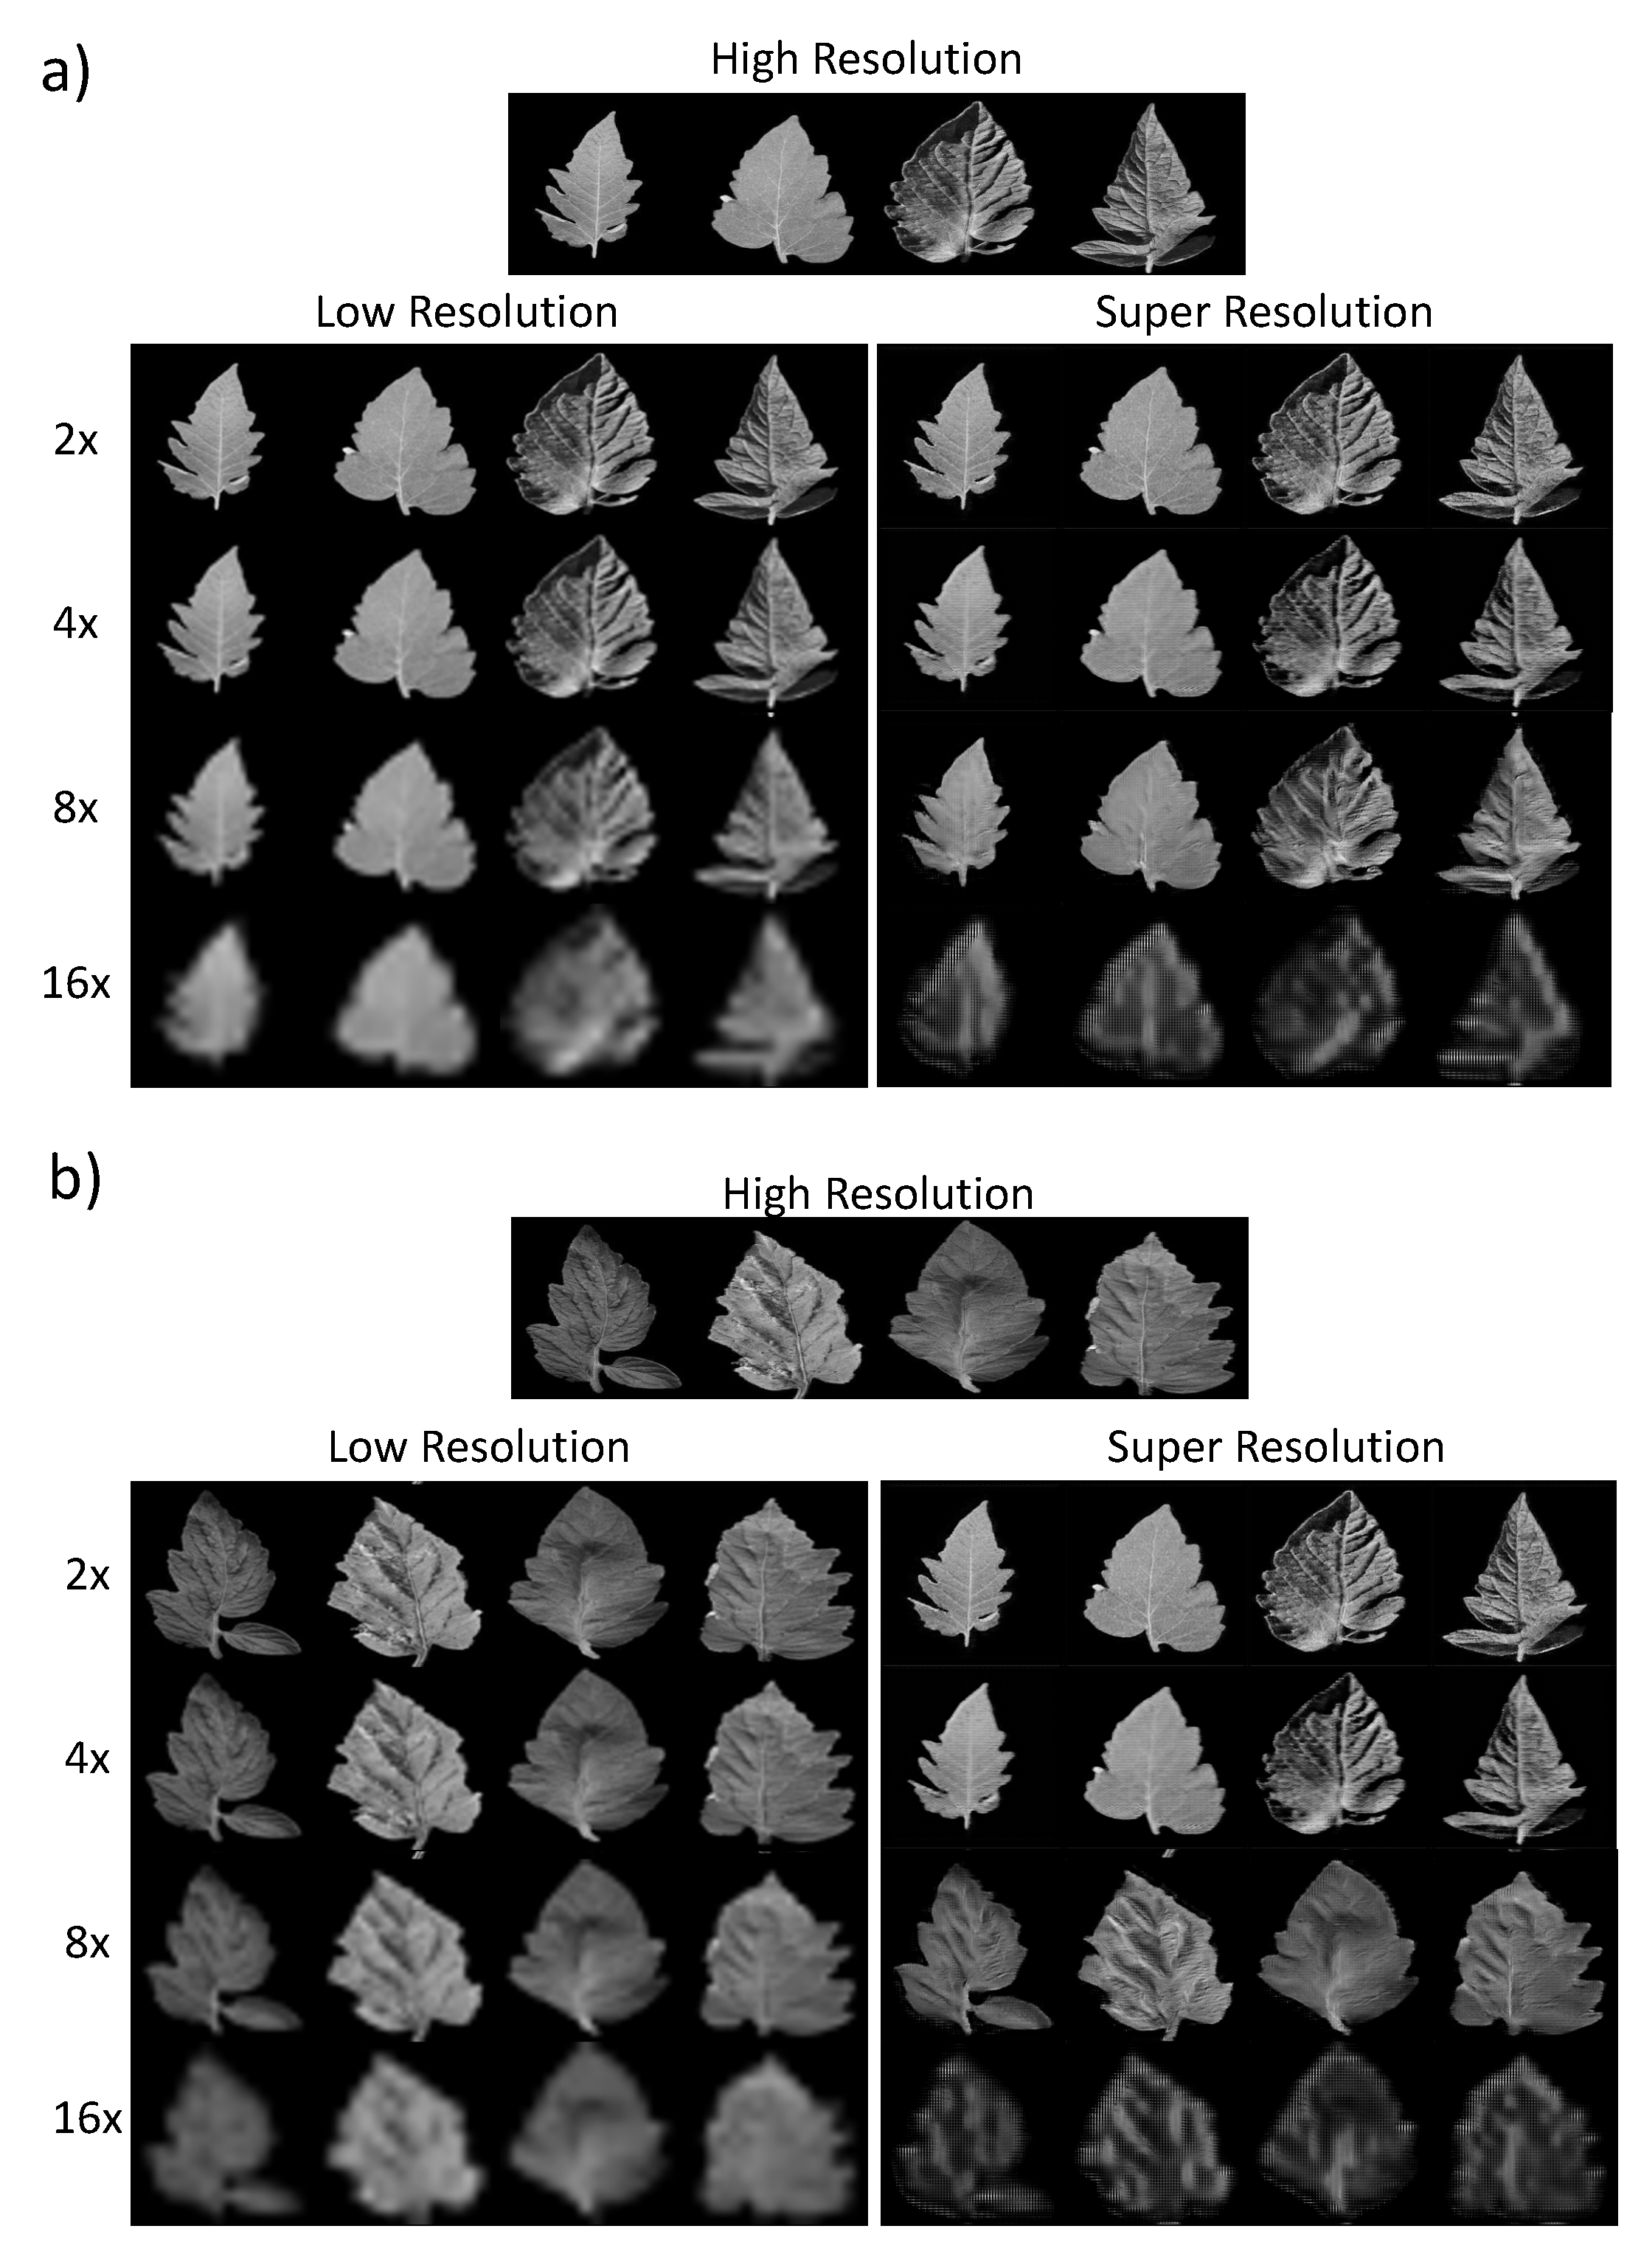
\includegraphics[scale=0.40]{results/srimages.pdf}
\end{center}
   \caption{a) Tomato - healthy. b) Tomato - bacterial spot} 
\label{fig:srimages}
\end{figure*}

\subsection{CT cores-SR}
\texttt{[THESE RESULTS MIGHT BE REMOVED]}
In this experiment, we use CT scans of two cores, one that contains only turface and other that contains roots and turface. Table~\ref{tab:results_cores} shows the classification accuracy in a test set (200 images per class). Figure~\ref{fig:srimages_cores} contains some examples of HR, LR and SR of each class (Turface+Roots and Turface).

\begin{table}[h]
\caption{Classification performance on the CT cores dataset applied to a test set.}
\label{tab:results_cores}
\centering
\begin{tabular}{|l|c|c|c|}
\hline
  Scale   & Accuracy & TP & TN \\
\hline
\hline
HR & 87.7 & 73.3 & 100 \\
\hline
LR2x & 86.4 & 72.8 & 100 \\
SR2x & \textbf{86.7} & \textbf{73.3} & 100 \\
\hline
LR4x & 81.5 & 63.0 & 100 \\
SR4x & \textbf{86.0} & \textbf{72.0} & 100 \\
\hline
LR8x & 54.9 & 09.5 & \textbf{100} \\
SR8x & \textbf{88.3} & \textbf{76.5} & 100 \\
\hline
LR16x & 50.3 & 00.0 & \textbf{100} \\
SR16x & \textbf{79.9} & \textbf{59.8} & 100 \\
\hline
\end{tabular}
\end{table}

\begin{figure*}[h]
\begin{center}
\includegraphics[scale=0.40]{results/srimages_cores.pdf}
\end{center}
   \caption{a) Turface+Roots. b) Turface}
\label{fig:srimages_cores}
\end{figure*}

\subsection{X-ray backscatter data-SR}

% See the dataset at http://gigadb.org/dataset/100346 
X-ray bacscatter technology allows scanning roots of plants non-destructively. We are currently working on the developing of a device to this end. Figure~\ref{fig:srtest} shows SR applied to this type of data.

\begin{figure*}[h]
\begin{center}
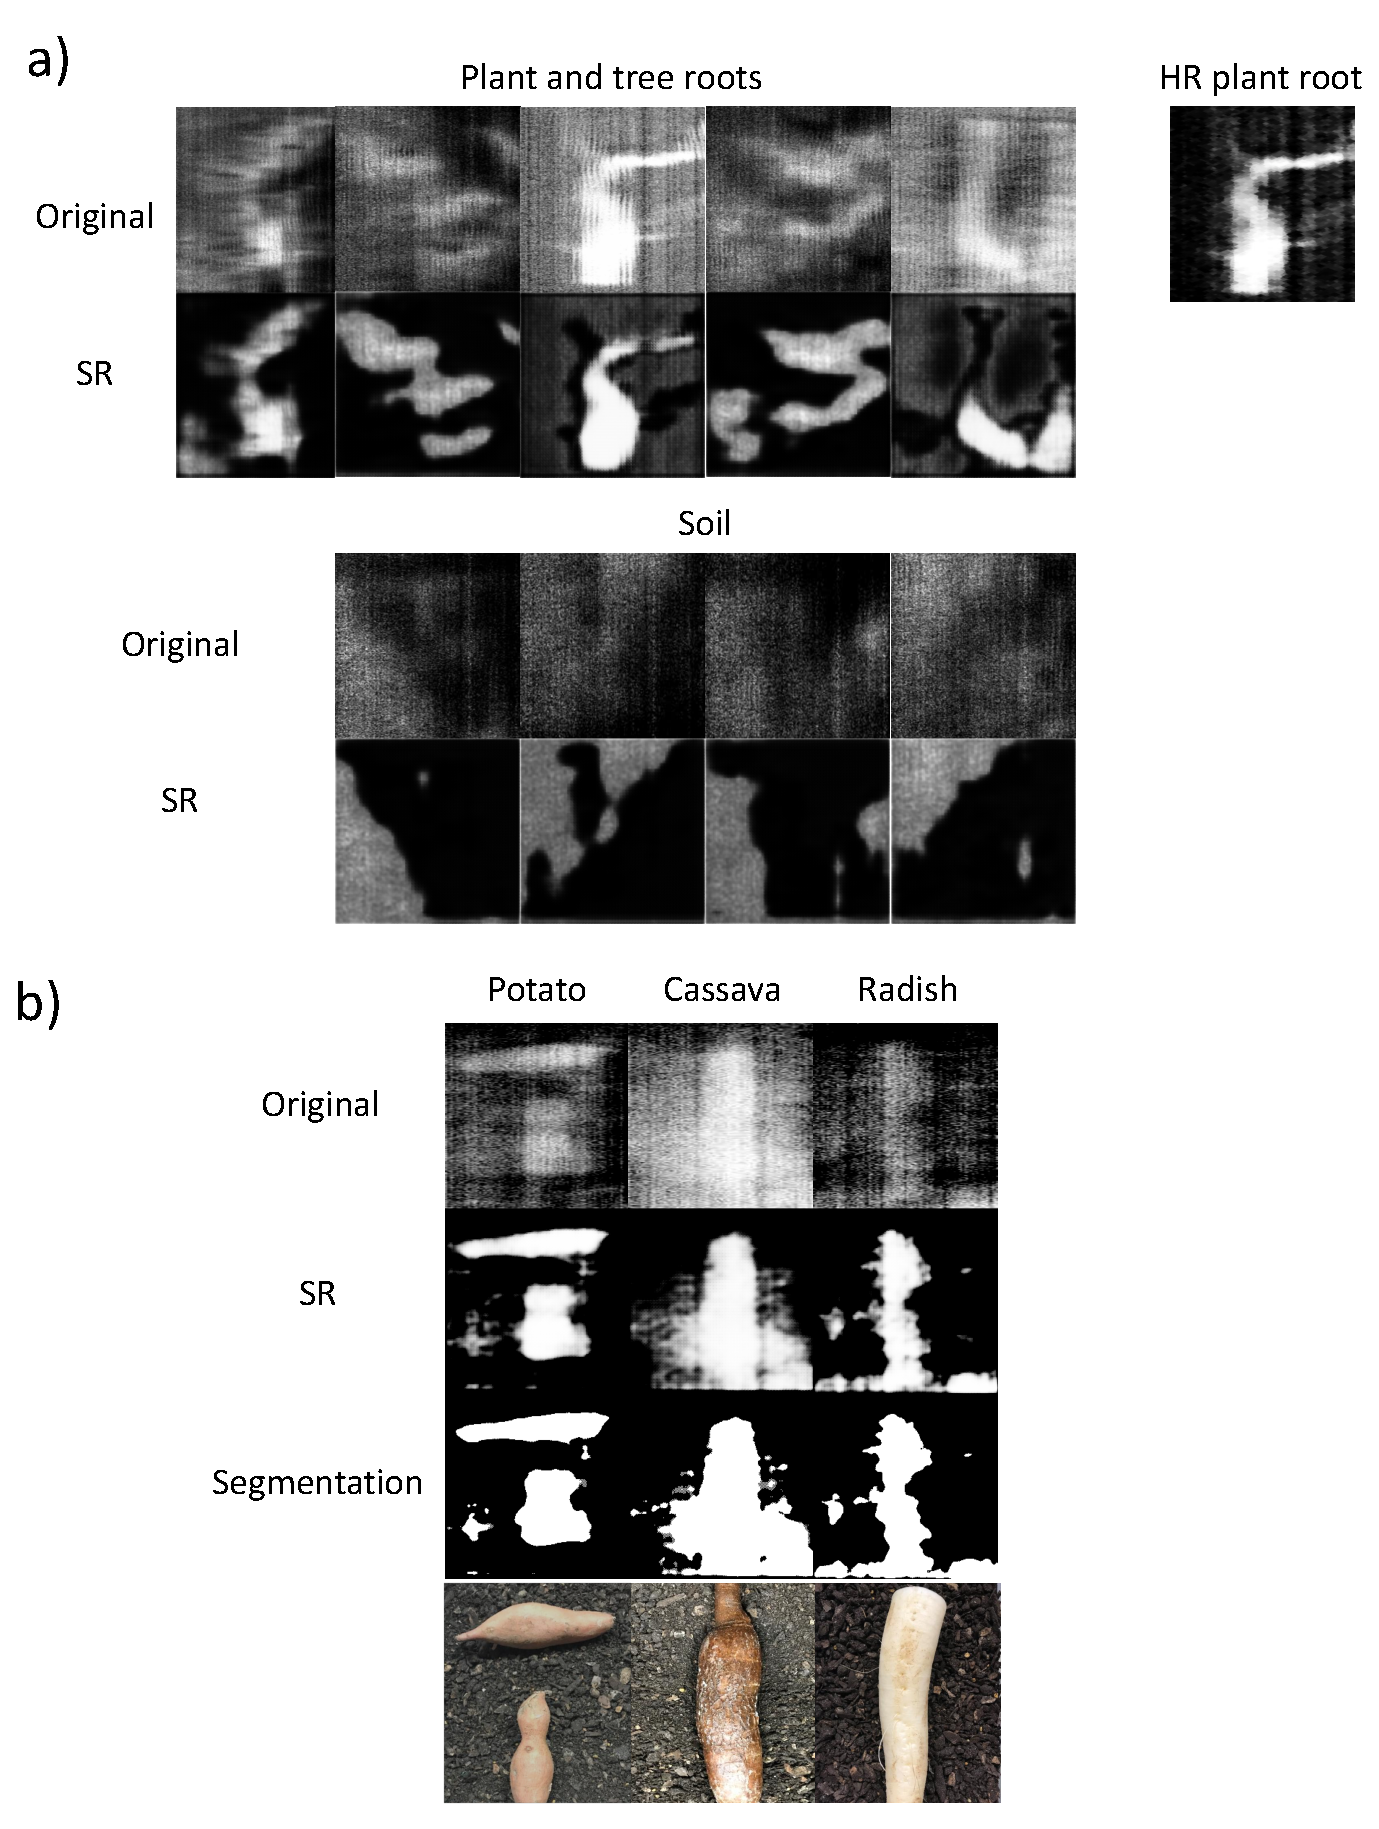
\includegraphics[scale=0.70]{results/srxray.pdf}
\end{center}
   \caption{SR applied to X-ray backscatter images. a) Training data; b) Test data}
\label{fig:srtest}
\end{figure*}

\section{Concluding remarks}

For applications where the data is acquired by different sensors, we recommend to train a classifier with a selected high-quality data set and use GANs to map the other data to the ``training domain.''

%\clearpage

{\small
\bibliographystyle{ieee}
\bibliography{egbib}
}

\end{document}
